\documentclass[a4paper]{article}

\usepackage[french]{babel}
\usepackage[T1]{fontenc}
\usepackage[utf8]{inputenc}
\usepackage{float}
\usepackage{amsmath}
\usepackage{graphicx}
\usepackage{wrapfig}
\usepackage{lscape}
\usepackage{rotating}
\usepackage{epstopdf}
\usepackage{multirow}
\usepackage{lmodern}
\usepackage[left=3cm, right=3cm, bottom=4cm, top=4cm]{geometry}
\usepackage{array}
\usepackage{pdfpages}
\usepackage{titlesec}
\usepackage{moreverb}  


\usepackage[gen]{eurosym}
\DeclareUnicodeCharacter{20AC}{\euro{}}

\usepackage{hyperref}
\hypersetup{
    colorlinks,
    citecolor=black,
    filecolor=black,
    linkcolor=black,
    urlcolor=black
}

\title{Document de planification initiale}

\author
{
    François {\sc Boschet}\\
    Arnaud {\sc Lods}\\
    Marlène {\sc Tuekam}\\
    Alexandre {\sc Bouchet}\\
    Guillaume {\sc Perrudin}\\
    Nguyen {\sc Song Hai}\\
    Romain {\sc Colombat}
}

\date{\today}

\newcommand{\pagevierge}[0]{\newpage\thispagestyle{empty}\null\newpage}

\begin{document}
    % Ouh c'est sale.
    \hypersetup{pageanchor=false}
    
\includepdf[pages=1]{figure/couv.pdf}
    \hypersetup{pageanchor=true}

    \newpage
    \thispagestyle{empty}
    \mbox{}

    \newpage
    % A decommenter pour la release
    \setcounter{tocdepth}{4}
    \tableofcontents
    \setlength{\parskip}{10pt}

    \newpage
    \thispagestyle{empty}
    \mbox{}

    \newpage
    
    
    \section{Introduction}
		
		\section{Rappel de la phase d'analyse}
\label{sec:rappel}
		
    \newpage
\section{Architecture générale}
\label{sec:generale}

Pour la réalisation de notre projet, nous allons utiliser des bases de données pour le stockage des données et pour la recherche, un serveur, des framework et une visionneuse de documents. La figure ci-dessous présente l'architecture logicielle générale de notre projet. Nous allons dans cette partie présenter la communication entre les différents modules de cette architecture.
    \begin{figure}[H]
        \centering
        \includegraphics[width=\textwidth]{figure/Archi.png}
            \caption{Architecture globale de la plateforme}
            \label{archi}
    \end{figure}

L'architecture se divise en deux grandes parties : serveur et client. 
Le serveur hébergeant l'application est un serveur Linux. Il comporte les modules suivants :
\begin{itemize}
	\item Le framework Laravel : il est utilisé pour le codage du centre de la plateforme web en PHP.
	\item La base de données MongoDB : c'est dans cette base que seront stockées toutes les données de l'application. Laravel pourra donc envoyer des requêtes pour modifier des données.
	\item La base de données ElasticSearch : cette base contiendra exactement les mêmes données que MongoDB et les requêtes de recherche y seront envoyées.
\end{itemize}

Le serveur communique avec le client à travers Laravel via un protocole HTTP. Côté client, nous allons utiliser le framework Bootstrap pour réaliser une interface graphique adaptées aux mobiles, tablettes et ordinateurs. Nous utiliserons également le plugin Openseadragon qui est une visionneuse pour la consultation de document. 

Nous allons détailler dans la suite la modélisation de chacun de ces modules de l'architecture générale du projet, ainsi que la communication entre ceux-ci.

    \newpage
\section{Architecture de la base de données}
\label{sec:bdd}

\subsection{Base de données}

Notre base de données est gérée par un système NoSQL : MongoDB. Nos données sont reparties par collections (c’est l’équivalent d’une table en SQL). Dans ces collections, les données sont écrites sous forme de document JSON. Le format JSON permet de représenter l’information de manière structurée. Un document JSON est composé de paires nom/valeurs ou de listes ordonnées de valeurs. Ces valeurs peuvent être des objets eux-mêmes représentés sous format JSON ; des tableaux ou des valeurs génériques : nombre, chaîne de caractère, booléen. 


Voilà un exemple de document que nous aurons dans la collection Revues : 


\begin{verbatimtab}[3]
{
	‘_id’ : 1,
	‘Nom’ : ‘Mai 68’,
	‘Description’ : ‘Ceci est une revue de presse sur Mai 68’,
	‘TitreArticles’ : [ 
		{ ‘idArticle’ : ‘34354’, ‘Titre’ : ‘Effervescence dans les universités françaises’ },
		{ ‘idArticle’ : ‘78e64a’,  ‘Titre’ :	‘Premières barricades de Mai 68’ }
  ]
}
\end{verbatimtab}

Chaque document dispose d’un id afin de pouvoir le retrouver rapidement. Cela permet aussi de pouvoir référencer d’autres objets de la base de données. 

Le diagramme suivant résume la modélisation de notre base de données :


\begin{figure}[H]
        \centering
        \includegraphics[scale=0.35]{figure/ModelBDD.png}
            \caption{Modélisation de la base de données}
            \label{fig:modelbdd}
\end{figure}

Certaines informations peuvent sembler répétitives comme la liste des articles favoris qui contient les mêmes informations que celles contenues dans les documents de la collection Article. Cependant, avec MongoDB, nous ne pouvons pas faire de jointure entre les tables. Si nous voulons les informations sur l’article, il sera nécessaire de faire une deuxième requête dans la base avec l’id du document de l’article pour obtenir ces informations. C’est pourquoi certaines informations sont dupliquées, notamment celles qui seront affichées. Cela permet d'économiser une requête à la base de données et donc du temps. Pour notre exemple, lors de l’affichage de la liste des favoris dans l’espace utilisateur, il est indiqué le titre, le titre du journal, la date et un extrait de l’article. 


Chaque flèche représente une référence, c’est-à-dire que l’id du document correspondant est stockée afin de pouvoir le retrouver dans la base. Les tableaux Coord[] stockent les coordonnées du  titre ou du mot. Cela nous permettra de le mettre en surbrillance lorsqu’il est l’objet de la recherche. 

\subsection{Elasticsearch}

Elasticsearch est un moteur de recherche, il nous servira pour rechercher parmi les articles de notre base, mais aussi pour n'importe quelle requête de recherche que nous aurons besoin de faire. Elasticsearch construit un index à partir des données afin de les parcourir rapidement et de manière optimisée. Pour notre projet, Elasticsearch indexera chaque collection de la base de données.  Cela nous dispense de construire nous-mêmes l'index de la base de données et les requêtes de recherche seront plus rapides que si nous les envoyions directement à MongoDB.


Habituellement, Elasticsearch dispose de sa propre base de données qu’il indexe. Nous utilisons donc le plugin elasticsearch-river-mongodb\cite{GitRiver}. Il permet à Elasticsearch d’utiliser une base de données MongoDB comme source de données. 


De plus, à chaque ajout, mise à jour ou suppression de données dans la base MongoDB, Elasticsearch met automatiquement à jour son index. Pour cela, il est nécessaire que la base MongoDB soit en \textbf{\textit{replica set}}.  Un \textbf{\textit{replica set}} est un groupe d’instances MongoDB qui maintiennent les mêmes données. Dans ce groupe, chaque instance est accessible en lecture et il y a une instance primaire qui est la seule à être accessible en écriture. Lorsque des modifications sont faîtes dans cette instance, les modifications sont répliquées aux autres instances du groupe. Dans notre cas, la base de données MongoDB sera l’instance primaire et Elasticsearch, par le biais du plugin, sera considérée comme une instance secondaire.


Pour effectuer une recherche dans la base à l’aide d’Elasticsearch, nous avons deux moyens. Soit nous pouvons utiliser l’API REST. Cette API utilise le format JSON pour les requêtes et les réponses et supporte les principales méthodes HTTP (GET, DELETE, PUT, POST). 


Elle est utilisée de la façon suivante :
\begin{verbatim}
http://host:port/[index]/[type]/[_action|id]
\end{verbatim}
Avec

\begin{itemize}
	\item index : Nom de l’index sur lequel porte l’opération
	\item type : Nom du type de document
	\item \_action : Nom de l’action à effectuer
	\item id : Identifiant du document
\end{itemize}


Par exemple, nous pourrons récupérer le document avec son id mais aussi effectuer une recherche d’un terme particulier :
\begin{verbatim}
http://host:port/[index]/[type]/_search?q=mai68
\end{verbatim}

Pour une recherche plus complexe, il faut envoyer une requête au format JSON :

\begin{verbatim}
{
    "query": {
        "bool": {
            "must": [
                {
                    "query_string": {
                        "default_field": "my_field",
                        "query": "text"
                    }
                }
            ],
            "must_not": [ ],
            "should": [ ]
        }
    },
    "from": 0,
    "size": 10,
    "sort": [ ]
}
\end{verbatim}

Avec
\begin{itemize}
	\item La partie \textit{must} contient les termes que doivent avoir les documents recherchés.
	\item La partie \textit{must\_not} les termes que le document ne doit pas contenir
	\item La partie \textit{should} les documents qui auront ces termes seront mis en haut de la liste
	\item \textit{from} correspond à l'indice du document par lequel vous voulez que la liste des résultats commence
	\item \textit {size} est le nombre de résultats que l'on veut récupérer
	\item \textit{sort} permet de trier les résultats
\end{itemize}
Il n'est pas nécessaire de tous les spécifier à chaque requête.


L’autre moyen est d’utiliser le plugin Head d’Elasticsearch. Il permet d’avoir accès à une interface. Depuis cette dernière, nous pouvons consulter l’état d’Elasticsearch et de ses index. Nous accédons aussi à une interface de moteur de recherche.

\subsection{Communication avec php}
\subsubsection{MongoDB}

Pour communiquer avec une base MongoDB, PHP dispose d’une classe Mongo. Celle-ci permet de faire des ajouts, des modifications et des suppressions dans la base de données. 

\begin{verbatim}
$m = new MongoClient();

// select a database
$db = $m->databaseName;   
$collection = $db->databaseCollection;

$collection->insert($doc);
\end{verbatim}

Le \textit{\$doc} aura été défini avant.

\subsubsection{Elasticsearch}

Pour Elasticsearch, nous utilisons le client PHP officiel pour Elasticsearch. Ainsi, nous pouvons envoyer des requêtes à Elasticsearch et récupérer les résultats de la recherche. Ces requêtes peuvent utiliser la même syntaxe qu’une requête de l’API REST. Par exemple, dans une base de données de restaurants :

\begin{verbatimtab}
$json = '{

    "query": {
        "bool": {
            "must": [
                {
                    "query_string": {
                        "default_field": "restau.borough",
                        "query": "Bronx"
                    }
                }
            ]
        }
    }
}';

$params = [
    'index' => 'resto',
    'type' => 'restau',
    'body' => $json
];

$results = $client->search($params);
print_r($results);
\end{verbatimtab}

\newpage
Bien évidemment, Elasticsearch retourne les résultats au format JSON. Les données sont donc converties en un format lisible par PHP :

\begin{figure}[H]
        \centering
        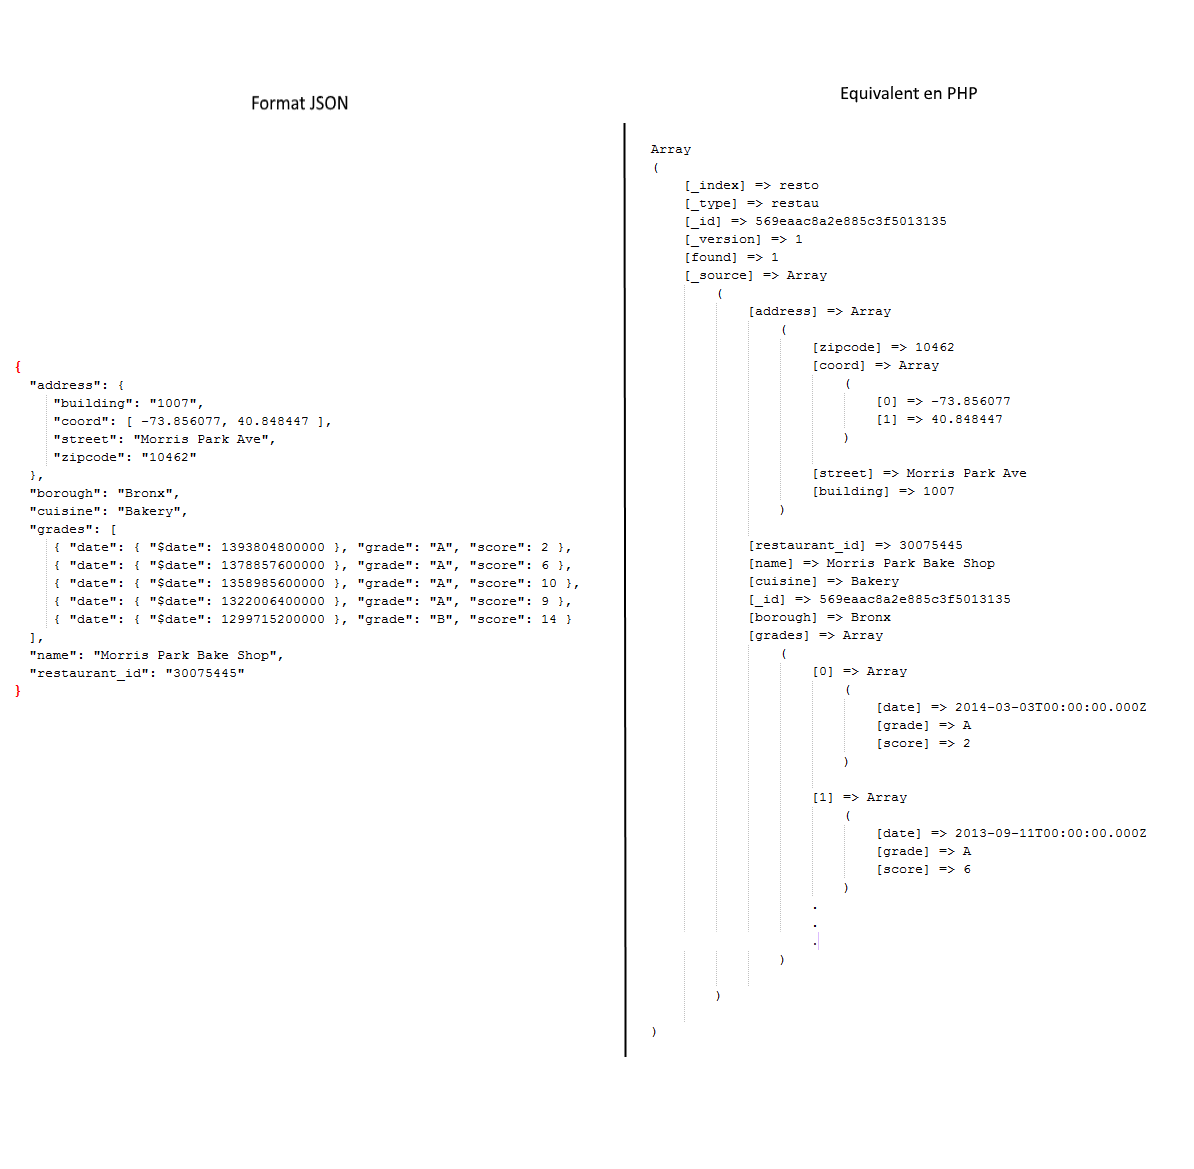
\includegraphics[width=\textwidth]{figure/dataJSONPHP.png}
            \caption{Format des données fournies par Elasticsearch}
            \label{fig:datajsonPhp}
\end{figure}

		\section{Architecture de Laravel}
\label{sec:laravel}

Laravel est un framework web PHP open-source. Nous allons utiliser ce Framework pour coder le cœur de l'application web. Il utilise le principe MVC ou modèle-vue-contrôleur. Ce framework permettra d'être plus efficace qu'en codant en PHP natif. Il intègre des fonctionnalités de routages et de mapping objet-relationnel entre autres. Les routes vont permettre de créer les différentes pages et sections de notre site du point de vue de l'URL. L'outil de mapping ORM utilisé par Laravel et nommé Eloquent va nous permettre d'interagir avec les différentes bases de données (MongoDB et Elasticsearch) à travers différents modèles PHP. C'est-à-dire que ce dernier va permettre une correspondance entre des objets et leurs données associées stockées sur la base de données.

\subsection{Les routes}

Les routes vont permettent de lier un url à une fonctionnalité de notre site. C'est à dire à une fonction précise d'un contrôleur.\\
Par exemple si nous souhaitons créer une page qui va lister tous les articles présents sur notre site, nous pouvons écrire dans le fichier route. Ici nous allons lier l'url http://www.notresite.extension/articles à la fonction index du contrôleur article.

\begin{verbatim}
Route::get('articles', 'ArticlesController@index');
\end{verbatim}

\subsection{Le contrôleur}

Le contrôleur est le cœur métier de notre application. Il va exécuter les tâches nécessaires à la requête demandée et transmettre ces informations à la vue.\\
Par exemple, ici nous allons récupérer tous les articles enregistrés et les passer à la vue "pages.articles". Pour cela, il faut tout d'abord communiquer avec le modèle "Article" en lien avec la base de données.

\begin{verbatim}
public function index()
{
	$articles = Article::all();
	return view('pages.articles', compact('articles'));
}
\end{verbatim}

\subsection{Le modèle}
Le modèle va permettre de définir des objets dans Laravel, par exemple, l'objet Article. Le modèle est en lien avec la base de données. Nous utilisons ici Elasticquent\cite{GitElasticquent} pour communiquer avec la base de données Elasticsearch et Moloquent\cite{GitLaravelMongo} pour communiquer avec MongoDB.

\begin{verbatim}
class Article extends Moloquent
{
	use ElasticquentTrait;
	protected $collection = 'article';
}
\end{verbatim}

\subsection{Les vues}

Le gestionnaire de vue de Laravel (nommé Blade) nous donne la possibilité de définir du code HTML à trou et qui inclue/hérite d'autres vues. Ici notre vue "pages.article" contient le code HTML de la vue article. Cette vue hérite de la vue globale définie par "app".
\paragraph{}
La vue globale contient la structure du site à inclure dans chaque page, c'est ici que nous faisons le lien avec Bootstrap et JQuery (utilisé par ce dernier). Nous incluons alors les fichiers CSS et Javascript nécessaires.

\begin{verbatim}
<!doctype html>
<html lang="fr">
<head>
	<meta charset="utf-8">
	<meta http-equiv="X-UA-Compatible" content="IE=edge">
	<meta name="viewport" content="width=device-width, initial-scale=1">
	<title>Gutemberg</title>
	<link href="https://maxcdn.bootstrapcdn.com/bootstrap/3.3.6/css/bootstrap.min.css" rel="stylesheet" integrity="sha256-7s5uDGW3AHqw6xtJmNNtr+OBRJUlgkNJEo78P4b0yRw= sha512-nNo+yCHEyn0smMxSswnf/OnX6/KwJuZTlNZBjauKhTK0c+zT+q5JOCx0UFhXQ6rJR9jg6Es8gPuD2uZcYDLqSw==" crossorigin="anonymous">
	@yield('css_includes')
</head>

<body>
	@yield('page_content')
	<script src="//code.jquery.com/jquery-1.12.0.min.js"></script>
	<script src="https://maxcdn.bootstrapcdn.com/bootstrap/3.3.6/js/bootstrap.min.js" integrity="sha384-0mSbJDEHialfmuBBQP6A4Qrprq5OVfW37PRR3j5ELqxss1yVqOtnepnHVP9aJ7xS" crossorigin="anonymous"></script>
</body>
</html>
\end{verbatim}

\begin{figure}[H]
        \centering
        \includegraphics[width=200px]{figure/diagrammeLaravel.png}
            \caption{Architecture Laravel autour des articles}
            \label{fig:datajsonPhp}
\end{figure}
		
    \section{Conclusion}
\label{sec:conclusion}
	
	Ce rapport et les deux présentations qui donnent suite à ce dernier représentent la fin de la phase d'analyse et de spécifications. Nous avons vu et estimé la durée de chacune des tâches pour chaque itération du projet. Cela nous a permis d'établir une planification initiale des tâches pour le reste du projet, du début de la phase de conception jusqu'au rendu de la dernière version du projet.

	L'étape suivante du projet sera donc la phase de conception de celui-ci. Nous établirons l'architecture de la base de données que nous utiliserons, nous définirons les différents modules de l'application, et la façon dont ceux-ci communiquent entre eux, et nous procéderons à l'installation de l'environnement de travail pour la suite du projet.
	
	%\newpage
	%\section{Annexes}
\label{sec:annexes}

	\begin{figure}[H]
        \centering
        
\includegraphics[width=\textwidth]{figure/gantt.png}
            \caption{Partie diagramme de Gantt}
            \label{fig:gantt}
    \end{figure}

    \begin{figure}[H]
        \centering
        
\includegraphics[width=\textwidth]{figure/gantt.png}
            \caption{Partie diagramme de Gantt}
            \label{fig:gantt}
    \end{figure}

    \begin{figure}[H]
        \centering
        
\includegraphics[width=\textwidth]{figure/gantt.png}
            \caption{Partie diagramme de Gantt}
            \label{fig:gantt}
    \end{figure}
	
	\bibliographystyle{plain}
    \bibliography{input/biblio}
    
    
    % Manoucherie incoming
    \pagevierge
    \ifthenelse{\isodd{\thepage}}
    {\pagevierge}
    {}
    
\includepdf[pages=2]{figure/couv.pdf}
    
    
\end{document}
